\section{Conceptual Model}
\label{conceptual_model}

\subsection{Component Model}

In conceptual model an agent is an independent computational unit that manages its own resources (CPU, memory, disk, sensors, etc).

We add to Tropos Model the concept of \textit{strategy}.

The strategy is a alternative way of achieving a goal (as in GORE) and a component in the architecture. Each goal correspond to a component. Each OR decomposition in the DGM should correspond to a additional component.

Plans are implemented by code in the strategy component.

By this we aim at creating an appropriate abstraction to allow composable architecture while keeping the traceability between the requirements and implementation at runtime.

An agent in the system has a repository of strategies that had all its runnable code. The agent have a model of that repository that it can use for reason about its capacities and plans. The agent can also insert and remove plans from its repository.

\begin{itemize}
  \item \textbf{Capability}: description of a kind of goal that an agent can perform. Its an interface description in the architecture. (e.g SUM a and b)
  \item \textbf{Strategy}:
  \item \textbf{Plan}: a plan is a Capability alternative implementation (e.g (SUM,a,b) => {a+b}). Its also a module in the architecture.
  \item \textbf{Plan Repository}: repository of know plans
\end{itemize}

\subsection{Strategy Selection}

To allow component based adaptation we propose a mechanist of strategy selection at runtime.
For a hight level of flexibility we propose that the selection mechanism in itself should be developed as components in the architecture.

At a low level an agent has the capability of fulfill goals. Inspired by component based frameworks like Rainbow we propose that the strategy to fulfill a goal should be chosen by means of a utility function\cite{garlan_rainbow:_2004}. That utility function should be responsible to calculate which available strategy will have a better contribution for softgoals.

The capacity and strategy should be as follows:

\item \textbf{<Fulfill Goals> Goal} the capability of fulfill generic goals.

\item \textbf{<Fulfill Goals> Strategy } strategy to fulfill goals by selecting available strategies and evaluating them with an utility function. Consist of 3 sub-goals:
  \begin{itemize}
    \item Find Matching Strategies
    \item Decide on Strategies
    \item Deploy the Selected Strategy
  \end{itemize}
\end{itemize}

And the following three strategies implement the previous 3 goals.

\begin{itemize}
  \item \textbf{<Find Local Matching Strategies> Strategy} accomplish <Find Matching Strategies>
  return the list of matching strategies. A matching strategy is any strategy that implement the goal interface.

  \item \textbf{<Select a Strategy> Strategy} accomplish <Decide on Strategies>
  use a pre-configured utility function that analyses strategies metadata and select a strategy.

  \item \textbf{<Deploy Strategy> Strategy} accomplish <Deploy the Selected Strategy>.
  Consist in deploying the chosen component.
\end{itemize}

\subsection{Runtime Model}

Dalpiaz et al. \cite{dalpiaz_runtime_2013} argue that traditional goal models are not enough for reason about the system at runtime. They  propose a distinction between Desgin-time Goal Model and Runtime Goal Model. We extend their proposal with model at runtime of the agent.

\begin{itemize}

\item \textbf{Goal Instance}: an actual instance of an objective for a given data set. (e.g SUM 2 and 3)

\item \textbf{Believe}: in the knowledge of an actor about itself and the context.

\end{itemize}

\begin{figure}
  \centering
  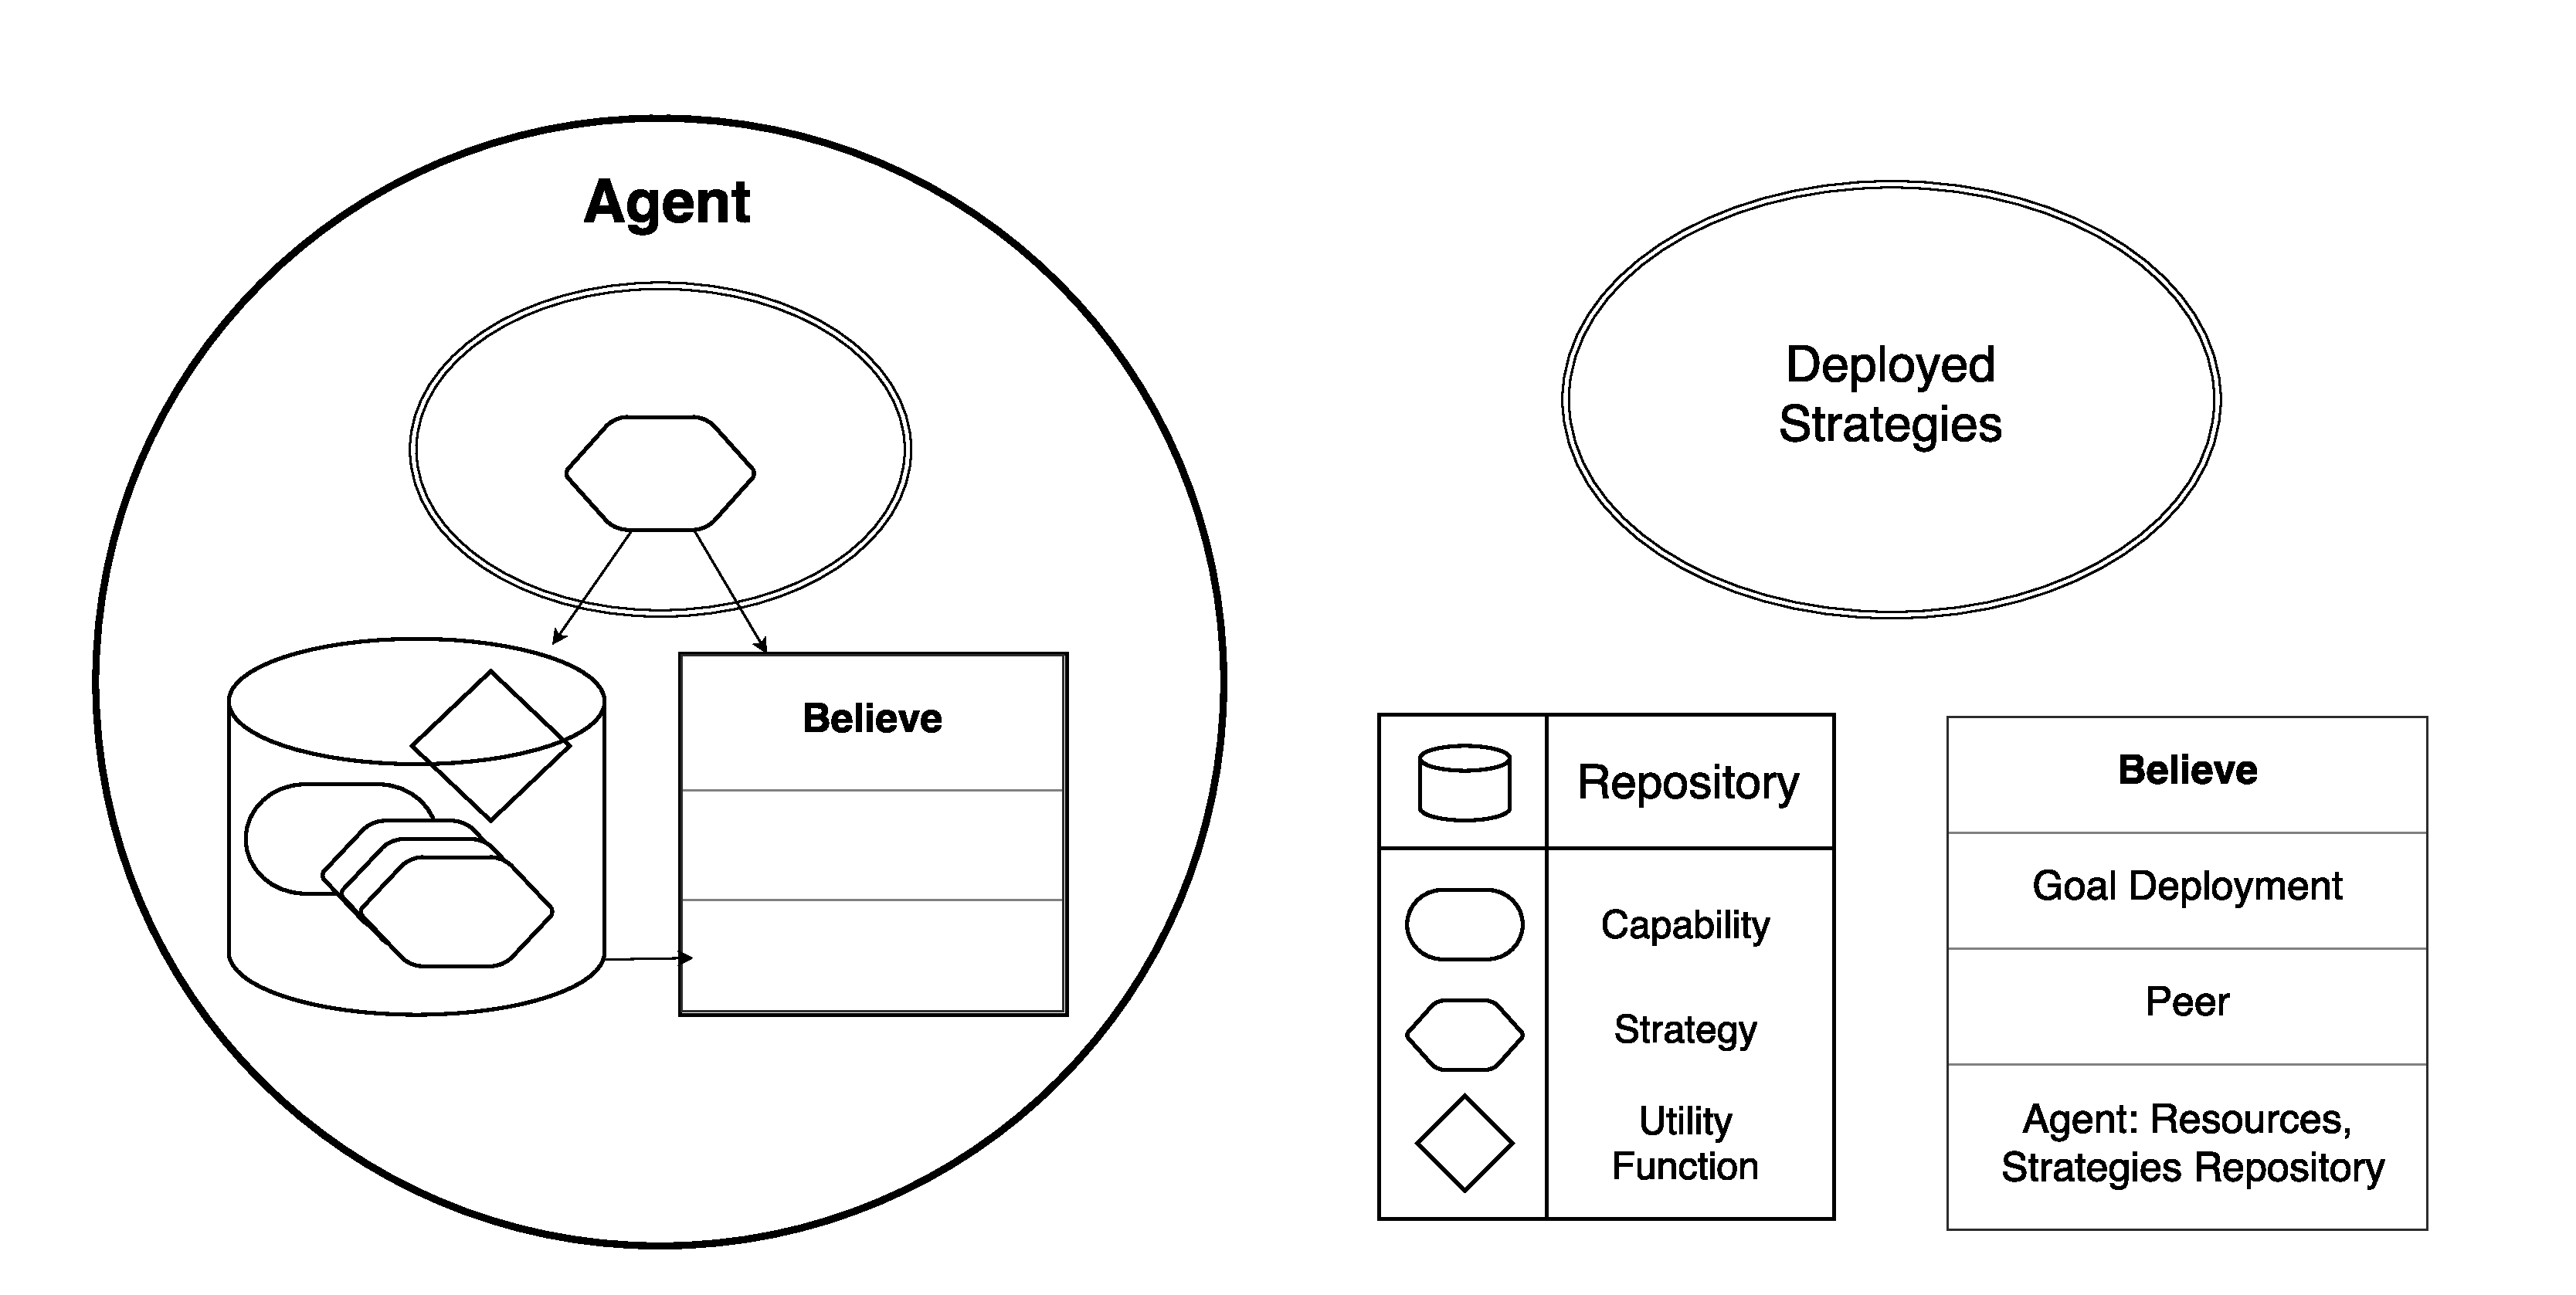
\includegraphics[width=\linewidth]{goalp-agent-repo-rcm-depl}
  \caption{Agent}
  \label{fig:goalp-agent}
\end{figure}

In the proposed model an actor achieve a goal by \emph{deploying a plan}. For instance the deployment of plan is a capability itself, as follows:

\begin{figure}
  \centering
  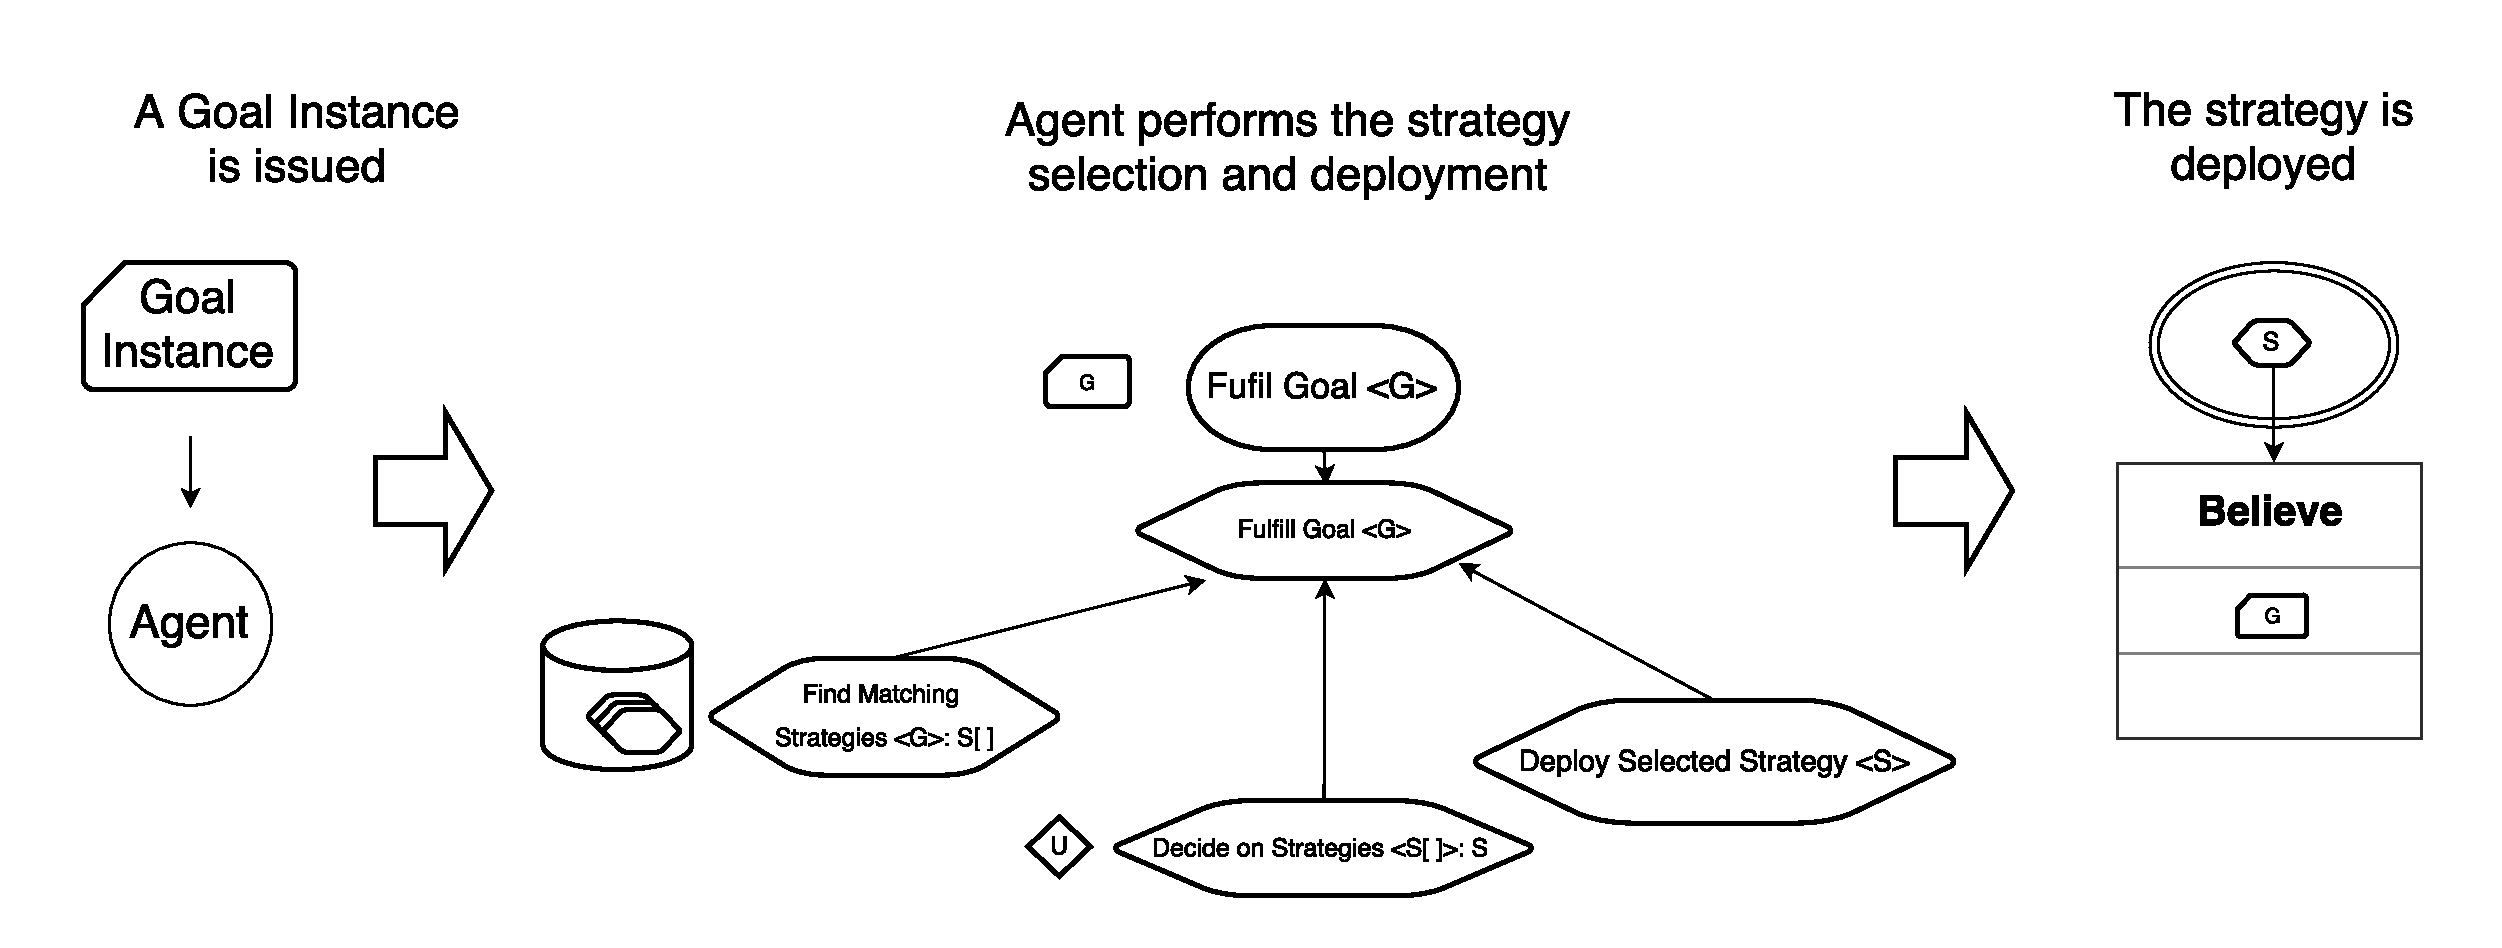
\includegraphics[width=\linewidth]{strategy_deployment}
  \caption{The deployment of a strategy}
  \label{fig:agent_composition}
\end{figure}

\begin{itemize}

\subsection{Awareness}

Self-awareness is provided by a set of self-awareness strategies. Example of self-aware strategies are:

\begin{itemize}
  \item \textbf{<List Local Strategies> Strategy} How the agent can know it actual capabilities.

  \item \textbf{<List Goal Instances> Strategy} How the agent can know it current intentions.

  \item \textbf{<List Deployed Strategies> Strategy} How the agent can know it current running strategies.

\end{itemize}


%
% \section{Resources}
%
% \section{Strategy Declaration}
%
%
% \section{Fault Model}
% Consistent/Inconsistent Failure
%
% Agent failure
%
% Resource failure
%
% Strategy failure
